\documentclass{article}
\usepackage{graphicx}
\usepackage{float}
\usepackage[a4paper, margin=2cm]{geometry}
\usepackage{titlesec}
\usepackage[font=small,labelfont=bf]{caption}
\usepackage{subcaption} % <— pour les sous-figures
\usepackage{booktabs}
\usepackage{siunitx}
\usepackage{tabularx}
\usepackage{amsmath, amssymb}
\usepackage{siunitx}
\usepackage{physics}    % pour \dv, \expval si tu veux (optionnel)
\sisetup{detect-all}
\sisetup{
  detect-all,
  separate-uncertainty,
  table-number-alignment = center,
  table-figures-integer = 3,
  table-figures-decimal = 3
}

\titleformat{\section}{\normalfont\large\bfseries}{\thesection}{1em}{}
\titleformat{\subsection}[block]{\centering\normalfont\normalsize\bfseries}{}{0pt}{}

\title{Rapport}

% Chemin commun aux images
\graphicspath{{rapport_image_divers/}}

\begin{document}

\maketitle

%--------------------------------------------------------------------POTENTIAL 1D--------------------------------------------------------------------
\section*{Environnement :}

% --- Figure avec deux sous-figures + une image pleine largeur ---
\begin{figure}[H]
  \centering
  \begin{subfigure}[c]{0.48\textwidth}
    \centering
    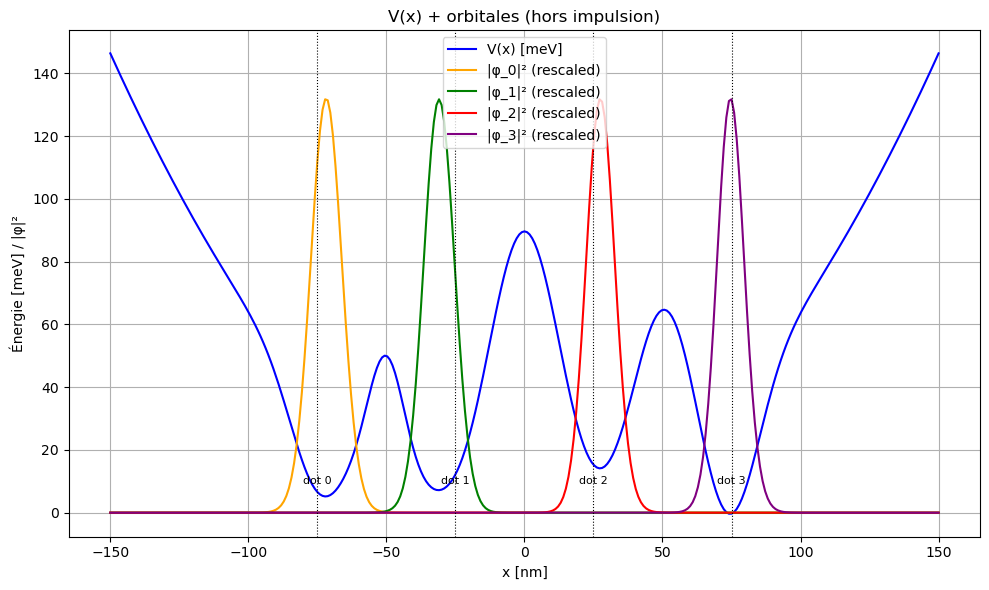
\includegraphics[width=\textwidth]{hors_impulsion_bon.png}
    \subcaption{Vue 1D hors impulsion}
    \label{fig:view_1D_off}
  \end{subfigure}\hfill
  \begin{subfigure}[c]{0.48\textwidth}
    \centering
    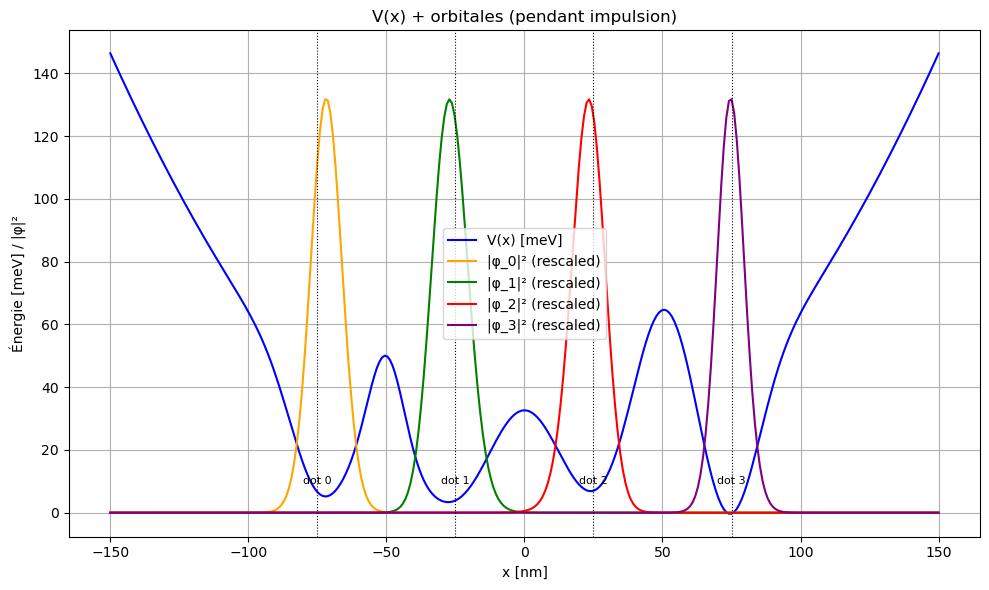
\includegraphics[width=\textwidth]{pdt_impulsion_bon.png}
    \subcaption{Vue 1D pendant impulsion}
    \label{fig:view_1D_on}
  \end{subfigure}
\end{figure}


%------------------------------------------------------CONSTRUCTION HEATMAPS------------------------------------------------------------

\section*{Construction des heatmaps :}
\begin{figure}[H]
  \centering
  \begin{minipage}[c]{0.6\textwidth}
    \centering
    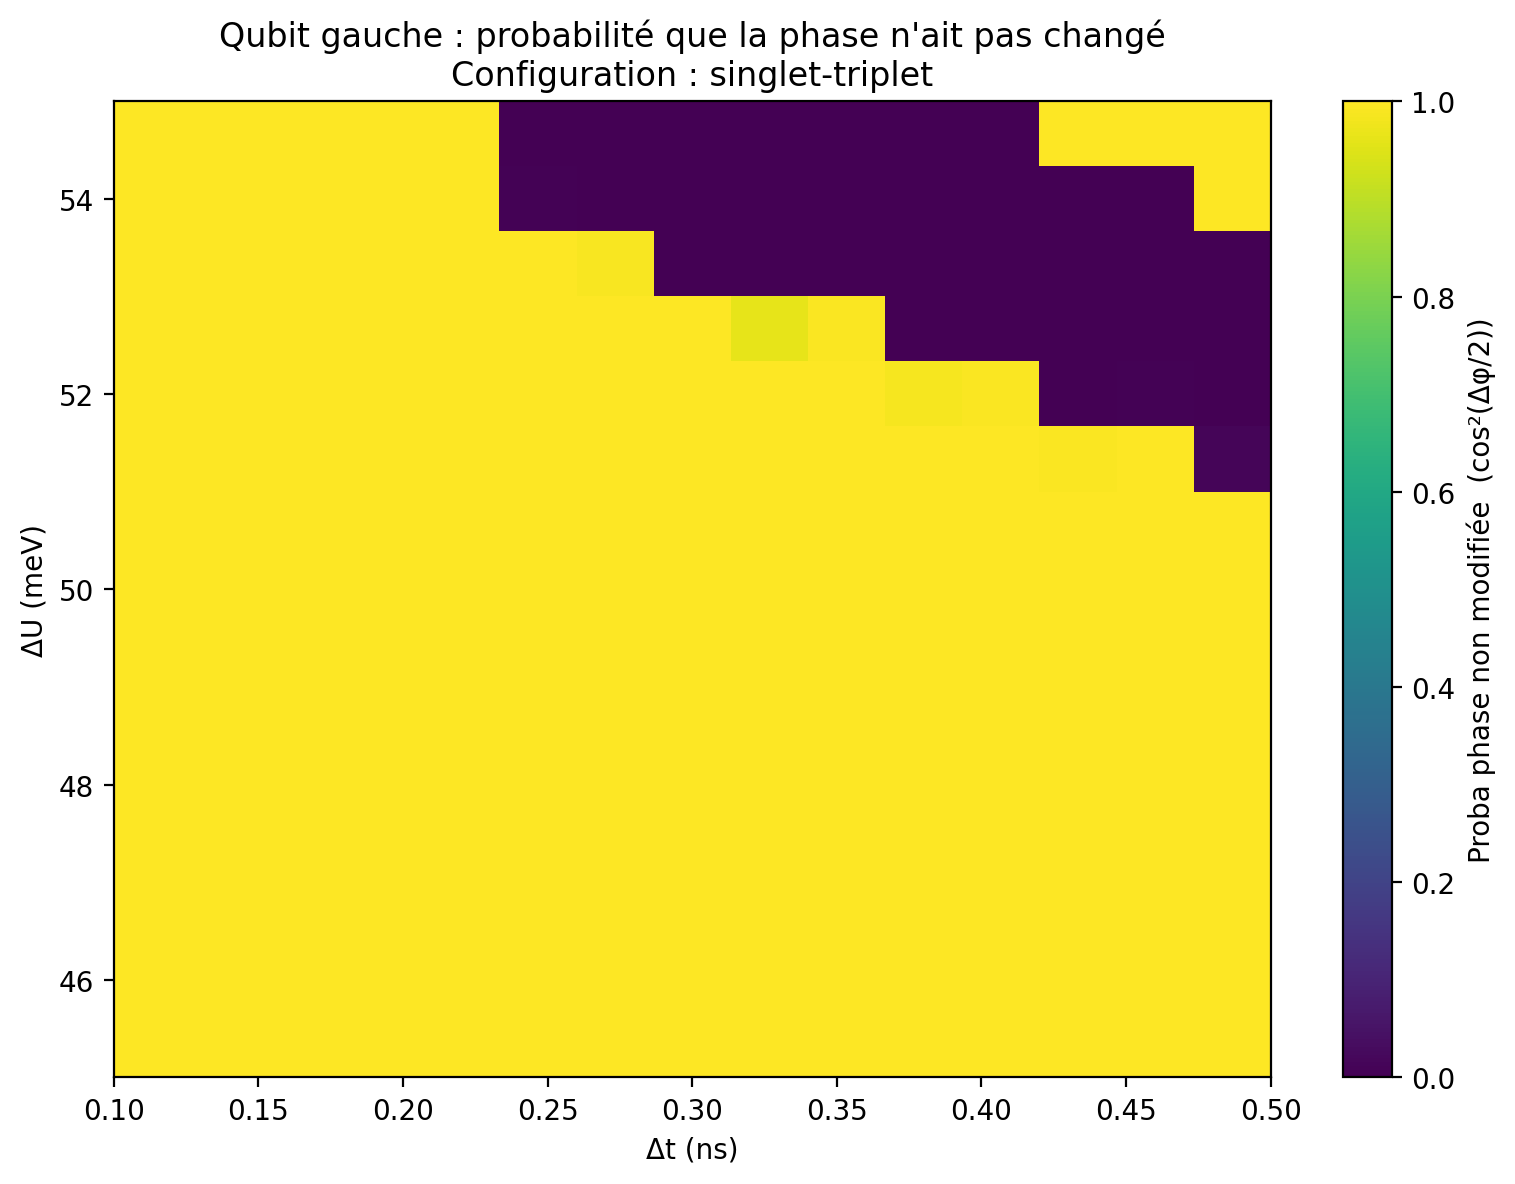
\includegraphics[width=0.5\textwidth]{qubit_results/singlet-triplet__p_si0_15_15/images/15x15__singlet-triplet__qubit/p_nochange_map_qubit_left_singlet-triplet_15x15_20250821-041033.png}
    \caption{Carte de fidélité de la phase du qubit.}
    \label{fig:fidelity_map_1}
  \end{minipage}\hfill
  \begin{minipage}[c]{0.6\textwidth}
    \centering
    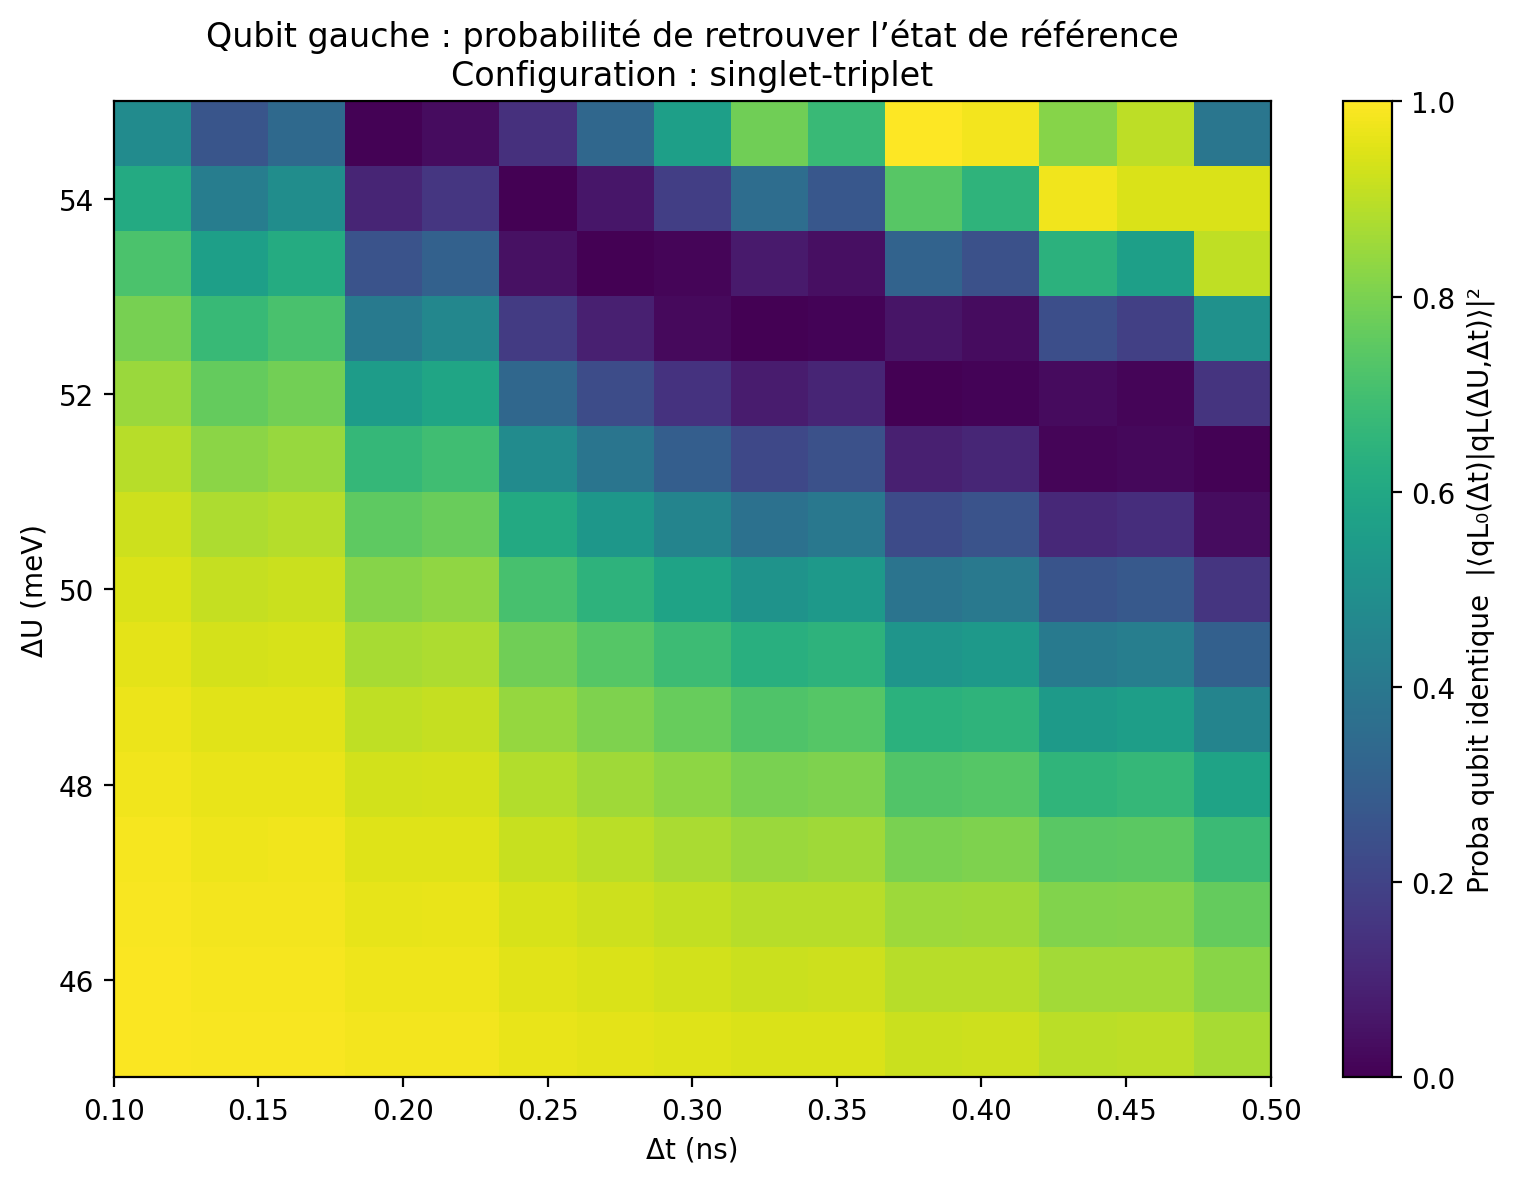
\includegraphics[width=0.5\textwidth]{qubit_results/singlet-triplet__p_si0_15_15/images/15x15__singlet-triplet__qubit/p_qubit_overlap_map_left_15x15_20250821-032340.png}
    \caption{Carte de fidélité de la phase du qubit.}
    \label{fig:fidelity_map_detector}
  \end{minipage}
\end{figure}

% === Dans le corps du document ===
\subsection*{Construction de la heatmap (récapitulatif mathématique)}

\subsubsection*{1. Grilles de balayage}
On balaye une grille rectangulaire $(\Delta U_i,\ \Delta t_j)$ :
\[
\Delta U_i \in [\Delta U_{\min},\Delta U_{\max}],\quad
\Delta t_j \in [\Delta t_{\min},\Delta t_{\max}],
\]
typiquement $\Delta U_i$ linéaire sur \si{\milli\electronvolt} et $\Delta t_j$ linéaire sur \si{\nano\second}.

\subsubsection*{2. Fenêtre d’impulsion lissée et hamiltonien dépendant du temps}
On déclenche une impulsion entre $t_0=t_{\mathrm{imp}}$ et $t_1=t_{\mathrm{imp}}+\Delta t$ via une fenêtre lissée
\[
w(t)=\tfrac{1}{2}\!\left[\tanh\!\Big(\tfrac{t-t_0}{\tau}\Big)-\tanh\!\Big(\tfrac{t-t_1}{\tau}\Big)\right],\qquad
0\le w(t)\le 1,
\]
avec $\tau$ une constante de lissage (dans le code, $\tau \approx (t_1-t_0)/30$).
L’Hamiltonien total est combiné comme
\[
H(t)=\big(1-w(t)\big)\,H_{\text{base}} \;+\; w(t)\,H_{\text{pulse}}(\Delta U,\Delta t).
\]

\subsubsection*{3. Potentiel effectif et orbitales localisées}
On construit un potentiel $V(x,t)$ à partir des paramètres géométriques (profondeurs de puits, barrières, etc.) et de la modulation $\Delta U$.
Pour $\Delta U=0$ on prend $V(x,t_0^-)$ (hors impulsion) ; pour $\Delta U\neq 0$, on
moyenne pendant l’impulsion :
\[
\overline{V}(x;\Delta U,\Delta t)=\frac{1}{t_1-t_0}\int_{t_0}^{t_1} V(x,t)\,dt.
\]
À partir de $\overline{V}$, on calcule les états propres 1-particule $\{\varphi_k(x)\}$ puis on
localise/quasi-diagonalise pour obtenir des orbitales de site $\{\phi_i(x)\}_{i=1..4}$.

\subsubsection*{4. Paramètres de Hubbard $t_{ij}$ et $U_i$ (2D effectif)}
À partir des orbitales localisées $\phi_i(x,y)=\phi_i(x)\,g(y)$ (gaussienne en $y$), on évalue :
\[
t_{ij}\;\simeq\;\matrixelement{\phi_i}{\hat{H}_{\text{sp}}}{\phi_j},
\qquad
U_i\;=\;\frac{e^2}{4\pi \varepsilon_0 \varepsilon_r}
\iint \frac{|\phi_i(\mathbf{r})|^2\,|\phi_i(\mathbf{r}')|^2}
{\sqrt{|\mathbf{r}-\mathbf{r}'|^2+a_{\text{soft}}^2}}\;d^2\mathbf{r}\,d^2\mathbf{r}'.
\]
Dans le code, ces intégrales sont réalisées par \texttt{t\_from\_orbitals} et
\texttt{U\_vector\_from\_orbitals}, avec adoucissement $a_{\text{soft}}>0$.

\subsubsection*{5. Évolution temporelle (TDSE) et état final}
On résout l’équation de Schrödinger dépendant du temps
\[
i\hbar\,\dv{t}\ket{\psi(t)}=H(t)\ket{\psi(t)},
\]
de $t=0$ à $T_{\text{final}}$, pour l’état initial $\ket{\psi(0)}=\ket{\psi_0}$ (ex. singlet–triplet préparé).
On ne conserve que l’état final $\ket{\psi_{\text{fin}}(\Delta U,\Delta t)}$.

\subsubsection*{6. Qubit droit : projection, phase relative et baseline}
On extrait le \emph{spinor} du qubit droit dans la base logique $\{\ket{S_R},\ket{T0_R}\}$ :
\[
a(\Delta U,\Delta t)=\braket{S_R}{\psi_{\text{fin}}},\qquad
b(\Delta U,\Delta t)=\braket{T0_R}{\psi_{\text{fin}}}.
\]
On définit la phase relative (enroulée dans $(-\pi,\pi]$)
\[
\phi(\Delta U,\Delta t)=\operatorname{wrap}\!\big(\arg a-\arg b\big).
\]
La \textbf{baseline} (référence) est la phase à $\Delta U=0$ pour chaque $\Delta t$ :
\[
\phi_0(\Delta t)=\phi(\Delta U{=}0,\Delta t).
\]

\subsection*{7. Deux cartes possibles}
\paragraph{(a) Carte “fidelity de phase” (utilisée dans ton code).}
On mesure la non–modification de phase par
\[
p(\Delta U,\Delta t)=\cos^2\!\left(\frac{\Delta\phi(\Delta U,\Delta t)}{2}\right),
\qquad
\Delta\phi(\Delta U,\Delta t)=\operatorname{wrap}\!\big(\phi(\Delta U,\Delta t)-\phi_0(\Delta t)\big).
\]
C’est cette grandeur $p\in[0,1]$ qui est affichée en \texttt{imshow} (axe $x:\ \Delta t$ en ns, axe $y:\ \Delta U$ en meV).

\paragraph{(b) Carte “overlap de spinor de référence”.}
On peut aussi comparer le spinor du qubit droit à celui de référence à \emph{même} $\Delta t$ (baseline en $\Delta U=0$) :
\[
p_{\text{ov}}(\Delta U,\Delta t)
=\Big|\braket{q_R^{(0)}(\Delta t)}{q_R(\Delta U,\Delta t)}\Big|^2,
\quad
\text{où}\ \ket{q_R}=\frac{1}{\sqrt{|a|^2+|b|^2}}\begin{bmatrix}a\\ b\end{bmatrix}.
\]

\subsection*{8. Rendu graphique}
On trace $p$ (ou $p_{\text{ov}}$) par interpolation bilinéaire minimale (ou spline si désiré), avec barre de couleur $\in[0,1]$, et étendue
\[
\text{extent}=\big[\Delta t_{\min}\!\times\!10^9,\ \Delta t_{\max}\!\times\!10^9,\ \Delta U_{\min},\ \Delta U_{\max}\big].
\]

\subsection*{9. Résumé pipeline (pseudo-code)}
\begin{align*}
\textbf{pour } \Delta U_i \ \textbf{et}\ \Delta t_j:\quad
&\overline{V}\Leftarrow \text{moyenne de }V(x,t)\ \text{pendant }[t_0,t_1] \\
&\{\phi_k\}\Leftarrow \text{orbitales localisées issues de } \overline{V} \\
&(t_{ij},U_i)\Leftarrow \text{intégrales sur }\{\phi_k\} \\
&H(t)\Leftarrow H_{\text{base}},H_{\text{pulse}} \text{ + fenêtre } w(t) \\
&\ket{\psi_{\text{fin}}}\Leftarrow \text{TDSE}(H(t),\ket{\psi_0}) \\
&(a,b)\Leftarrow \text{projection qubit droit} \\
&\phi\Leftarrow \operatorname{wrap}(\arg a-\arg b),\quad
\Delta\phi\Leftarrow \operatorname{wrap}(\phi-\phi_0) \\
&p=\cos^2\!\big(\tfrac{\Delta\phi}{2}\big)\quad\text{(ou }p_{\text{ov}}\text{)}
\end{align*}

\noindent\textit{Remarques pratiques.} 
(i) Pour $\Delta U=0$, la baseline $\phi_0(\Delta t)$ peut être évaluée une seule fois puis réutilisée.
(ii) Les cartes “coarse” $(N_U,N_T)$ peuvent être interpolées sur une grille plus fine si besoin.
(iii) Le poids dans le sous-espace logique du qubit droit est $\mathrm{weight}=|a|^2+|b|^2$ ; on renormalise $[a,b]^\top$ si nécessaire avant l’overlap.


%------------------------------------------------------ESSAI 1 ------------------------------------------------------------

\section*{1er essai avec une asymétrie :}

\begin{table}[H]
  \centering
  \caption{Paramètres de la simulation}
  \label{tab:params}
  \begin{tabularx}{0.95\linewidth}{
      >{\raggedright\arraybackslash}p{4cm}
      >{\raggedright\arraybackslash}p{2.5cm}
      S[table-format=3.3]
      >{\raggedright\arraybackslash}X
  }
    \toprule
    \textbf{Symbole / Nom} & \textbf{Unité} & \textbf{Valeur} & \textbf{Description} \\
    \midrule

    \multicolumn{4}{l}{\textbf{Profondeurs des puits}} \\[0.3em]
    Puit 0 & \si{\milli\electronvolt} & 30 & Énergie du puit gauche \\
    Puit 1 & \si{\milli\electronvolt} & 5  & Énergie du 2\ieme{} puit \\
    Puit 2 & \si{\milli\electronvolt} & 20  & Énergie du 3\ieme{} puit \\
    Puit 3 & \si{\milli\electronvolt} & 40 & Énergie du puit droit \\

    \addlinespace[0.6em]
    \multicolumn{4}{l}{\textbf{Hauteurs des barrières}} \\[0.3em]
    Barrière 0 & \si{\milli\electronvolt} & 35 & Hauteur gauche \\
    Barrière 1 & \si{\milli\electronvolt} & 80 & Hauteur centrale \\
    Barrière 2 & \si{\milli\electronvolt} & 60 & Hauteur droite \\

    \addlinespace[0.6em]
    Largeur des puits    & \si{\nano\metre} & 23    & Largeur typique \\
    Largeurs barrières   & \si{\nano\metre} & (15,40,30) & Largeurs respectives \\
    \bottomrule
  \end{tabularx}
\end{table}


\subsection{Heatmap des variations de phase du qubit et du détecteur}

\subsubsection{Singlet-Triplet :}

\begin{figure}[H]
  \centering
  \begin{minipage}[c]{0.48\textwidth}
    \centering
    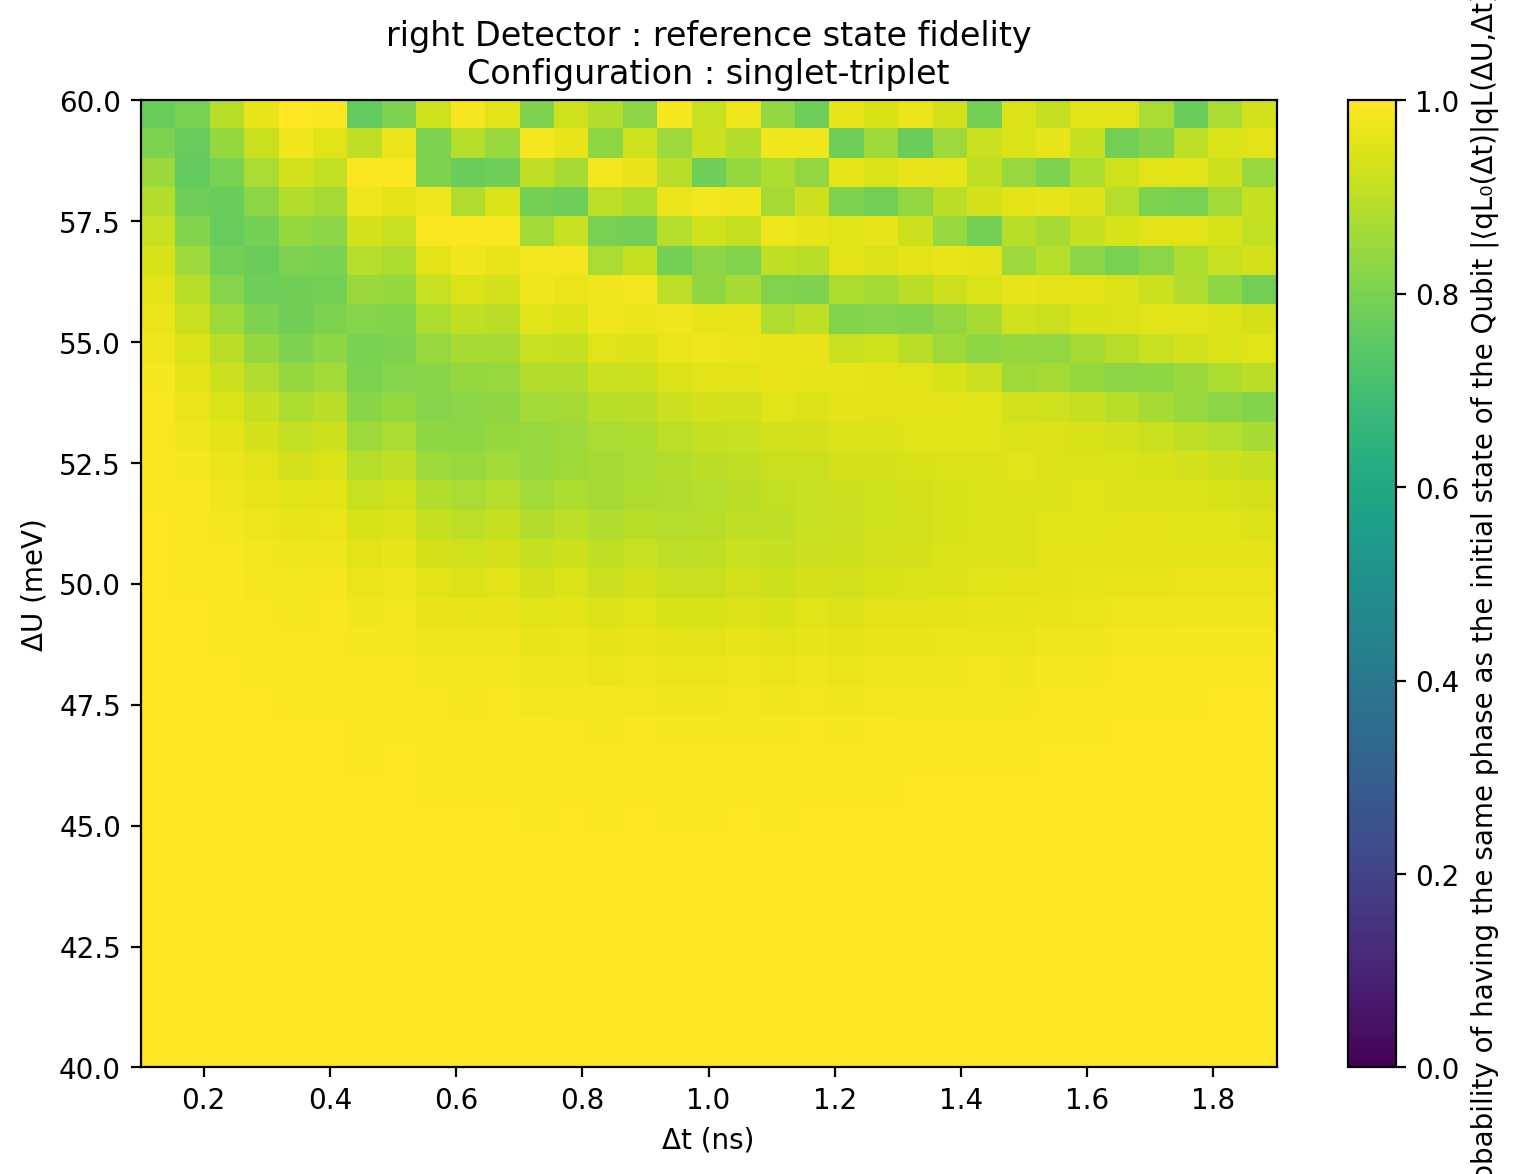
\includegraphics[width=\textwidth]{p_detector_overlap_map_33x33_20250822-003725_faible.png}
    \caption{Carte de fidélité (détecteur A)}
    \label{fig:fidelity_map_a}
  \end{minipage}\hfill
  \begin{minipage}[c]{0.48\textwidth}
    \centering
    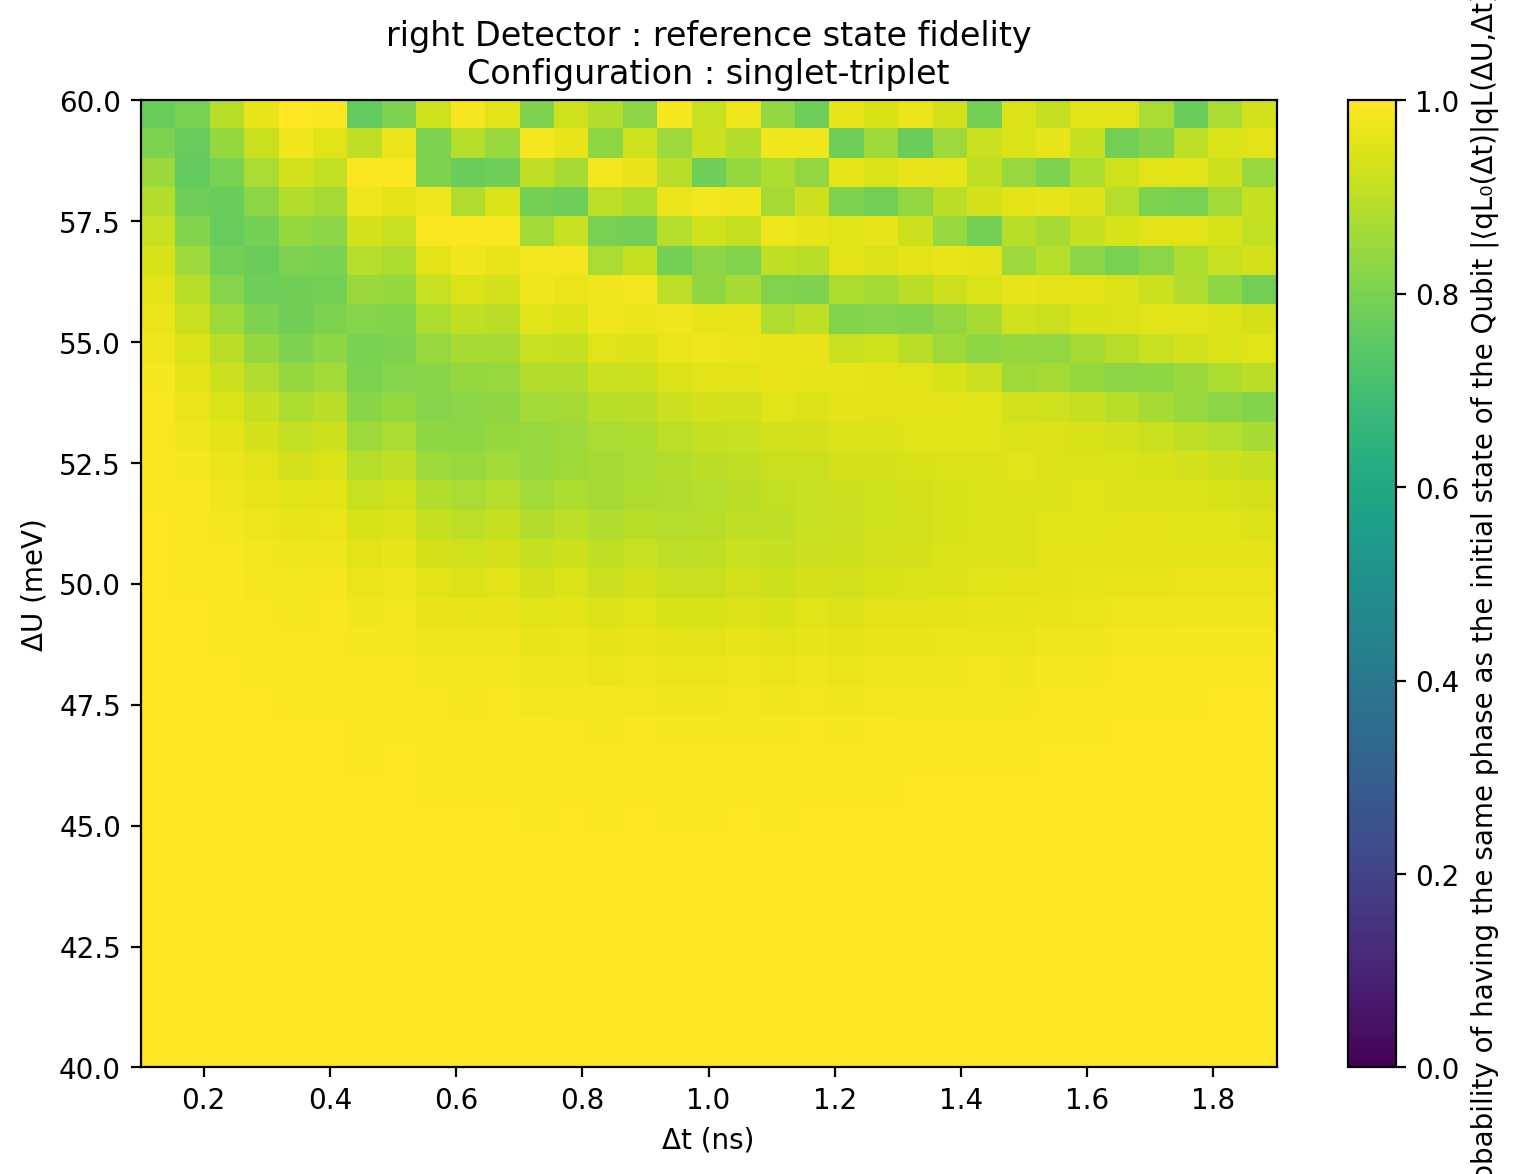
\includegraphics[width=\textwidth]{p_detector_overlap_map_33x33_20250822-003725_faible.png}
    \caption{Carte de fidélité (détecteur B)}
    \label{fig:fidelity_map_b}
  \end{minipage}
\end{figure}

\subsubsection{Triplet-Singlet :}
\subsubsection{Singlet-Singlet :}
\subsubsection{Singlet-Singlet :}


%------------------------------------------------------ESSAI 2 ------------------------------------------------------------

\section*{2ieme essai avec une asymétrie :}
% --- Figure simple (1 image) ---
\begin{table}[H]
  \centering
  \caption{Paramètres de la simulation}
  \label{tab:params}
  \begin{tabularx}{0.95\linewidth}{
      >{\raggedright\arraybackslash}p{4cm}
      >{\raggedright\arraybackslash}p{2.5cm}
      S[table-format=3.3]
      >{\raggedright\arraybackslash}X
  }
    \toprule
    \textbf{Symbole / Nom} & \textbf{Unité} & \textbf{Valeur} & \textbf{Description} \\
    \midrule

    \multicolumn{4}{l}{\textbf{Profondeurs des puits}} \\[0.3em]
    Puit 0 & \si{\milli\electronvolt} & 30 & Énergie du puit gauche \\
    Puit 1 & \si{\milli\electronvolt} & 5  & Énergie du 2\ieme{} puit \\
    Puit 2 & \si{\milli\electronvolt} & 5  & Énergie du 3\ieme{} puit \\
    Puit 3 & \si{\milli\electronvolt} & 40 & Énergie du puit droit \\

    \addlinespace[0.6em]
    \multicolumn{4}{l}{\textbf{Hauteurs des barrières}} \\[0.3em]
    Barrière 0 & \si{\milli\electronvolt} & 35 & Hauteur gauche \\
    Barrière 1 & \si{\milli\electronvolt} & 90 & Hauteur centrale \\
    Barrière 2 & \si{\milli\electronvolt} & 50 & Hauteur droite \\

    \addlinespace[0.6em]
    Largeur des puits    & \si{\nano\metre} & 23    & Largeur typique \\
    Largeurs barrières   & \si{\nano\metre} & (15,30,25) & Largeurs respectives \\
    \bottomrule
  \end{tabularx}
\end{table}


\begin{figure}[H]
  \centering
  \begin{minipage}[c]{0.48\textwidth}
    \centering
    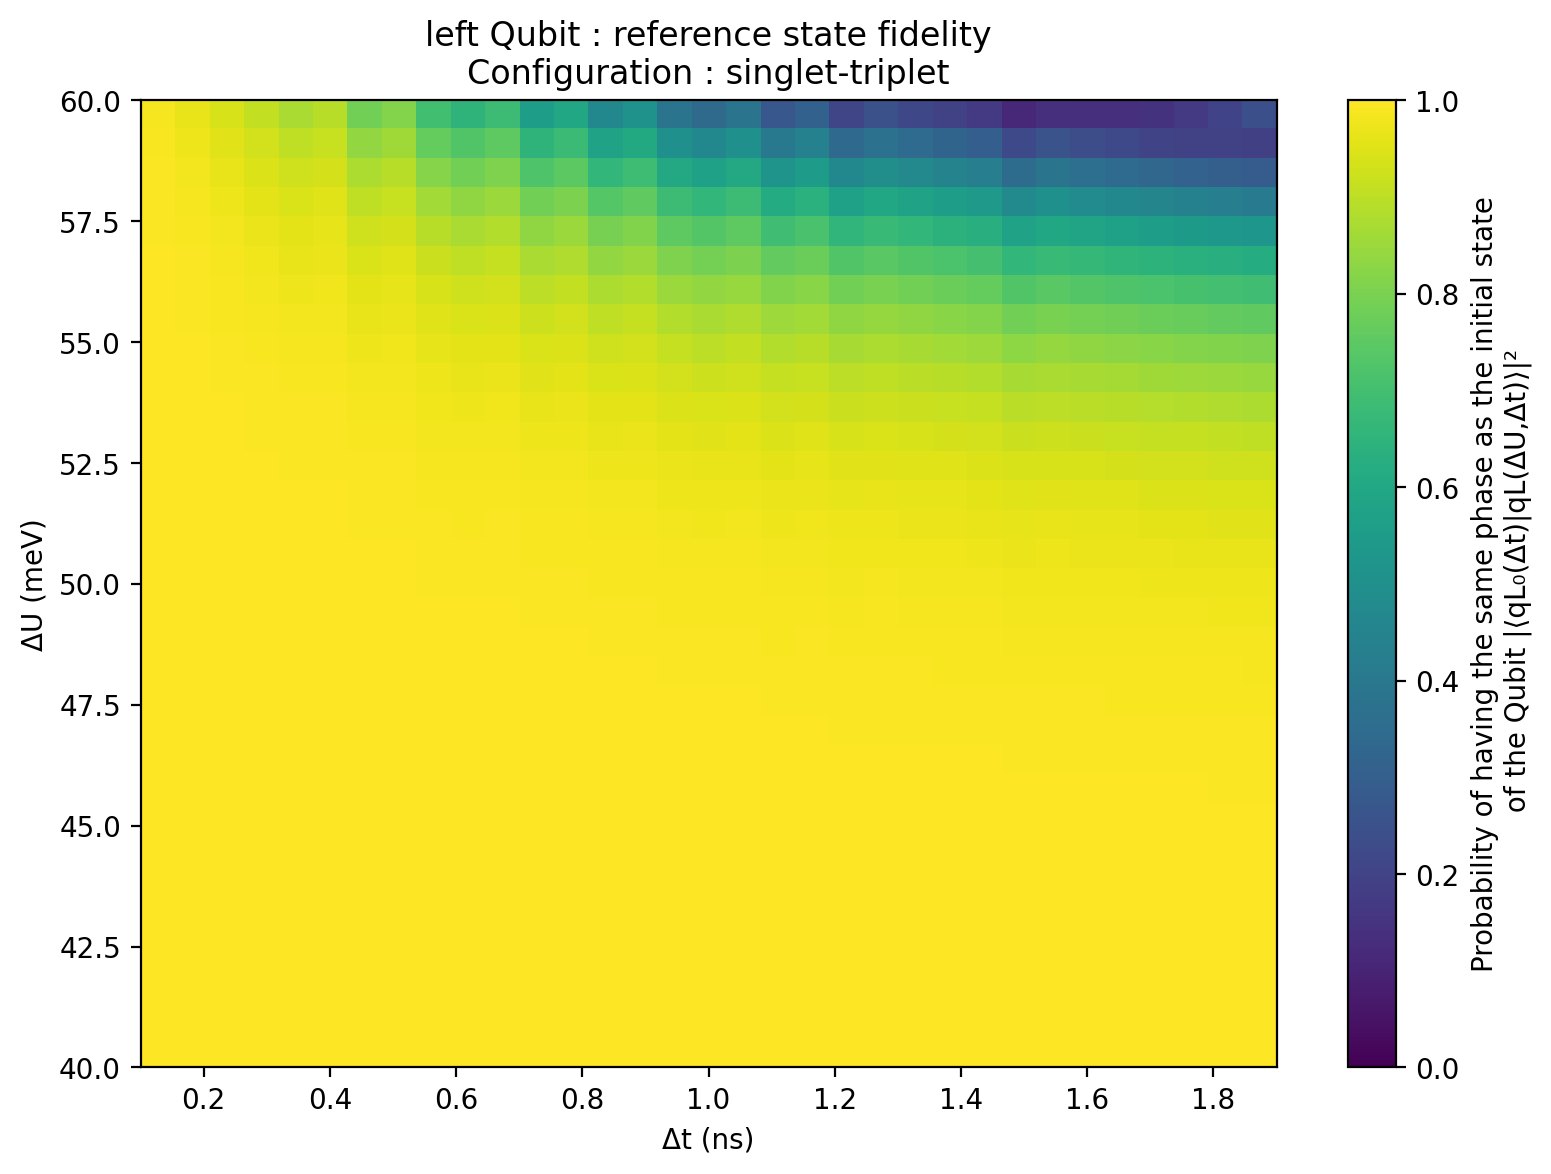
\includegraphics[width=\textwidth]{p_qubit_overlap_map_left_33x33_20250822-064424.png}
    \caption{Carte de fidélité (détecteur A)}
    \label{fig:fidelity_map_a}
  \end{minipage}\hfill
  \begin{minipage}[c]{0.48\textwidth}
    \centering
    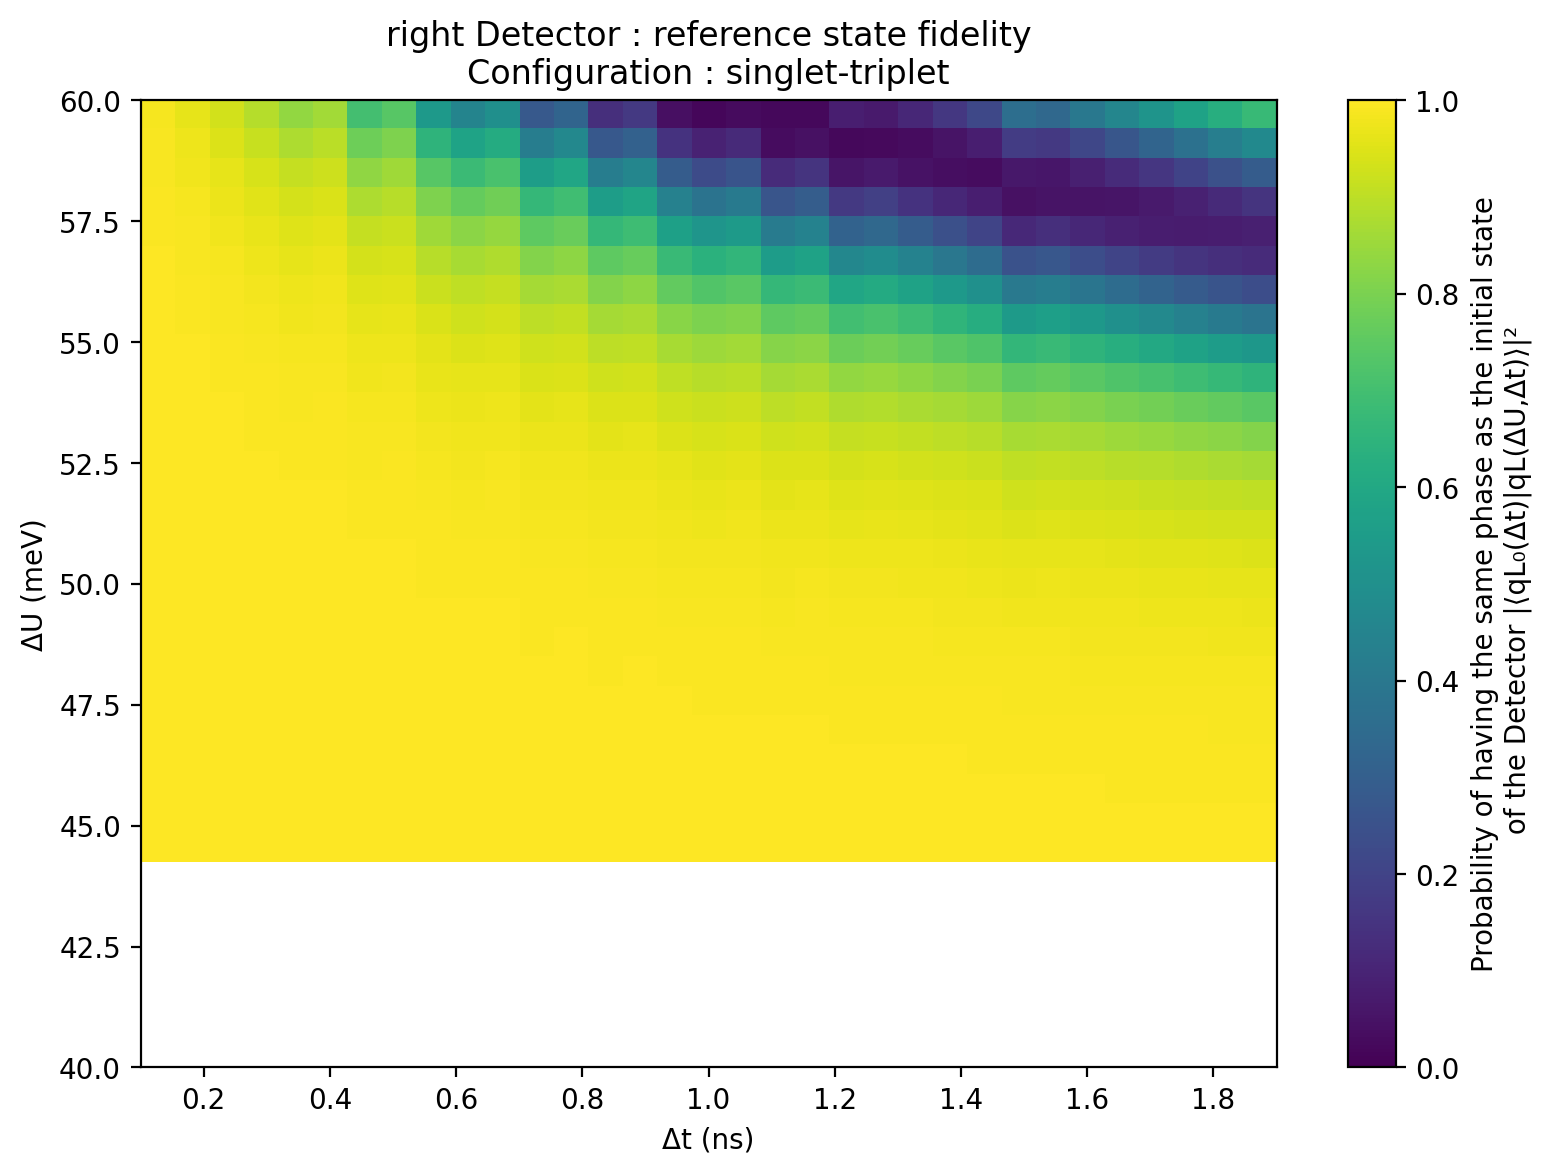
\includegraphics[width=\textwidth]{p_detector_overlap_map_33x33_bon_singlet-triplet.png}
    \caption{Carte de fidélité (détecteur B)}
    \label{fig:fidelity_map_b}
  \end{minipage}
\end{figure}

\subsection{essai avec DU=57meV et dt=1.2ns :}
\begin{figure}[H]
  \centering
  \vspace{0.8em}
    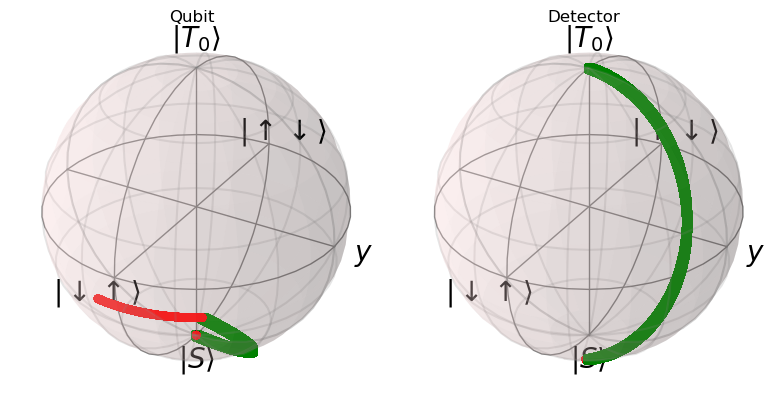
\includegraphics[width=0.6\textwidth]{singlet-triplet_du_57_dt_1_2_version1.png}
  \caption{Affichage sur les sphères de bloch}
  \label{fig:fidelity_map_detector}
\end{figure}


\section{The end :}

\subsection{Paramètres généraux :}
\begin{table}[H]
  \centering
  \caption{Paramètres de la simulation (issus de \texttt{param\_simu.py})}
  \label{tab:params}
  \begin{tabularx}{0.95\linewidth}{
      >{\raggedright\arraybackslash}p{4cm}
      >{\raggedright\arraybackslash}p{2.5cm}
      S[table-format=3.3]
      >{\raggedright\arraybackslash}X
  }
    \toprule
    \textbf{Symbole / Nom} & \textbf{Unité} & \textbf{Valeur} & \textbf{Description} \\
    \midrule
    $N_{\text{sites}}$       & — & 4 & Nombre de puits (dots) \\
    $N_{e}$                  & — & 4 & Nombre d’électrons \\
    $m_{\text{eff}}$         & $m_e$ & 0.067 & Masse effective (GaAs) \\
    $x_{\text{dots}}$        & \si{\nano\metre} & $\{-75,-25,25,75\}$ & Positions des 4 puits (x) \\
    $a$                      & \si{\milli\electronvolt\per\nano\metre\squared} & 6.5e-3 & Courbure du potentiel en $x$ \\
    Profondeurs puits        & \si{\milli\electronvolt} & (30, 5, 5, 40) & Énergies des 4 puits \\
    Hauteurs barrières       & \si{\milli\electronvolt} & (35, 90, 50) & Hauteurs des 3 barrières \\
    Largeur des puits        & \si{\nano\metre} & 23 & Largeur typique des puits \\
    Largeurs barrières       & \si{\nano\metre} & (15, 30, 25) & Largeurs des barrières \\
    $\sigma_x$               & \si{\nano\metre} & 15 & Largeur gaussienne en $x$ \\
    $\sigma_y$               & \si{\nano\metre} & 15 & Largeur gaussienne en $y$ (eff.) \\
    $y_{\text{confinement}}$ & \si{\milli\electronvolt\per\nano\metre\squared} & 0.1 & Confinement harmonique $y$ \\
    $t_{\text{imp}}$         & \si{\nano\second} & 0.1 & Instant de début de l’impulsion \\
    $\Delta t$               & \si{\nano\second} & 1.6 & Durée de l’impulsion \\
    $T_{\text{final}}$       & \si{\nano\second} & 2.0 & Temps total de simulation \\
    $\Delta U$               & \si{\milli\electronvolt} & 57 & Variation de $U$ due à l’impulsion \\
    $N_t$                    & — & 300 & Nombre de pas de temps \\
    $N_x$                    & — & dépend de la grille & Taille de la grille adaptative en $x$ \\
    $N_y$                    & — & dépend de la grille & Taille de la grille adaptative en $y$ \\
    \bottomrule
  \end{tabularx}
\end{table}


\end{document}
